\chapter{Flexible diffusion modelling of long videos}
\label{ch:fdm}

We have described the flexible diffusion paradigm, but challenges remain in applying it to complex and high-dimensional data. In this chapter we will explore and tackle these challenges with a focus on the video domain, in which data is both complex and high-dimensional. More precisely, we will describe two major contributions. The first is to apply diffusion models to video generative modelling, which by itself yields significantly better photorealism than prior work. The second is a tweak to the flexible diffusion framework that enables flexible generative modelling of videos up to a thousand frames long. The models we train can be conditioned on e.g. the first frame, last frame, a series of key frames, combinations of these, or any other set of frames. As well as enabling such flexible conditioning, we show that our flexible diffusion approach improves upon standard diffusion-based approaches in terms of sample quality.

To explain why flexible diffusion can bring such benefits, we point out that, prior to the work described in this chapter, there already existed methods for modelling short photo-realistic videos (e.g. 30 frames~\citep{weissenborn2019scaling}, 48 frames~\cite{clark2019adversarial} or 64 frames~\citep{ho2022video}). There did not exist methods for generating longer videos that are both coherent and photo-realistic, which we believe is a much harder challenge. One major difficulty is scaling: photorealistic image generative models~\citep{child2020very,dhariwal2021diffusion} are already close to the memory and processing limits of modern hardware.  A long video is at very least a concatenation of many photorealistic frames, implying resource requirements, long-range coherence notwithstanding, that scale with frame count. Attempting to model such long-range coherence makes the problem harder still, especially because in general every frame can have statistical dependencies on other frames arbitrarily far back in the video. And while deep generative models based on recurrent neural networks (RNN) theoretically impose no such conditional independence assumptions, in practice they must be trained over short sequences~\cite{gruslys2016memory,saxena2021clockwork} or with truncated gradients~\citep{tallec2017unbiasing}.  Despite this, some RNN-based video generative models have demonstrated longer-range coherence, albeit without yet achieving convincing photorealistic video generation~\citep{saxena2021clockwork,babaeizadeh2021fitvid,denton2018stochastic,kim2019variational,babaeizadeh2017stochastic}.


\begin{figure}[t]
    \centering
    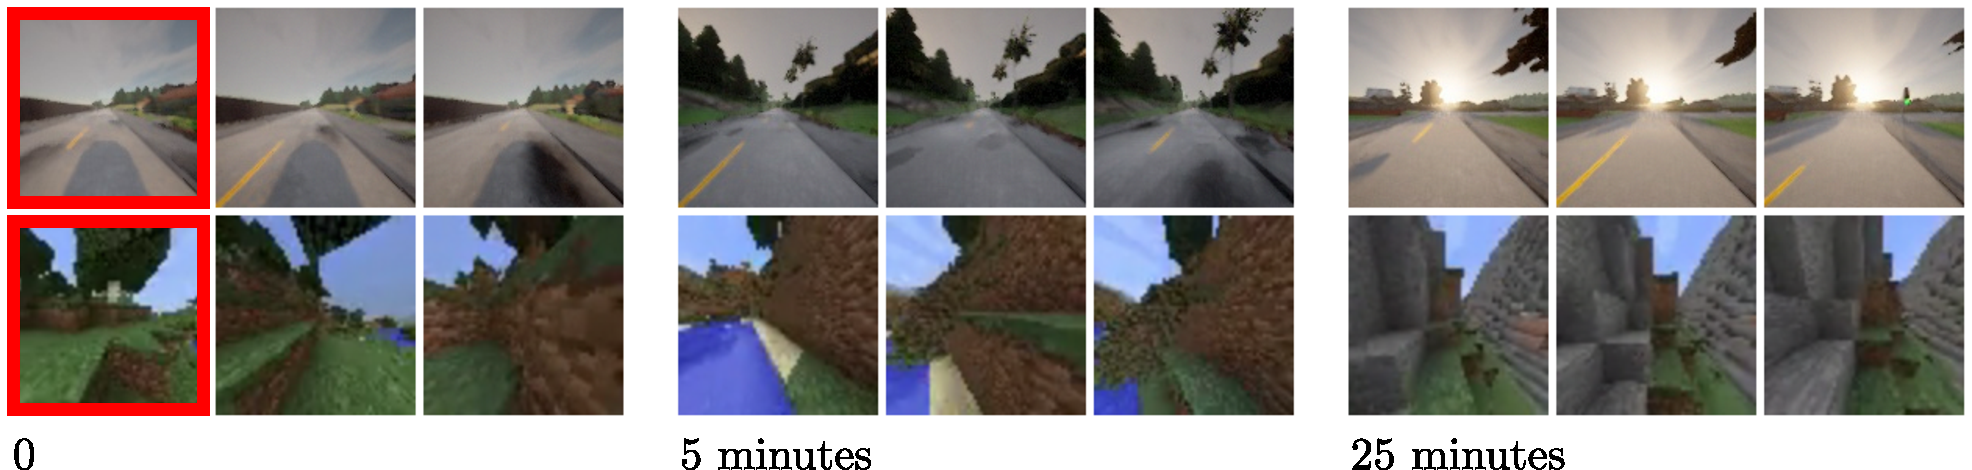
\includegraphics[width=\textwidth]{figs/fdm/fig1.pdf}
    \caption{A long video (25 minutes, or approximately 15\,000 frames) generated by FDM for each of CARLA Town01 and MineRL, conditioned on 500 and 250 prior frames respectively. We show blocks of frames from three points within each video, starting from the final observed frame on the left. Blocks are marked with the time elapsed since the last observation and frames within them are one second apart. We observe no degradation in sample quality even after $>15\,000$ frames.}
    \label{fig:fdm-1}
\end{figure}

To enable such convincing long video generation, 
we concurrently developed one of the first diffusion-based video generative models~\cite{ho2022video,yang2022diffusion,voleti2022mcvd}. While we see that straightforwardly applying DMs with a suitable architecture can yield improved photorealism versus previous methods, doing so does not automatically solve the problems of modelling long-range dependencies. DMs can still only model a limited number of frames at a time, and so techniques like autoregressive roll-outs are needed to extend them to long videos. Unfortunately, fixed-lag autoregressive models impose unrealistic conditional independence assumptions (the next frame being independent of frames further back in time than the autoregressive lag is problematic for generating videos with long-range coherence).  

In addition to imposing these unrealistic conditional independence assumptions, autoregressive models make flexible generation difficult. They are typically designed to enable unconditional generation, and their design also makes conditioning on the first frame or set of frames simple. Other forms of conditioning, however, become difficult, in particular conditioning on frames towards the end of the video.

In this work we embrace the fact that finite architectures will always impose conditional independence assumptions and prevent us from conditioning on all that we might desire. The question we ask is: given an explicit limit $K$ on the number of video frames we can jointly model, how can we best allocate these frames to generate a video of length $N > K$? In the unconditional case, one option is to use the previously-described autoregressive model but, if $K=N/4$, we could instead follow \citet{ho2022video} by training two models: one which first samples every 4th frame in the video, and another which (in multiple stages) infills the remaining frames conditioned on those. The latter option will enable new capabilities, like conditioning on frames further from the start of the video than the autoregressive model is able to condition on. It will also be able to capture dependencies across a larger time horizon. A downside is that is will not enable conditioning on both of the first two frames, as a purely autoregressive approach would.

The diffusion model which we propose in this chapter can sample any subset of video frames conditioned on observed values of any other subset of video frames, as long as the total size of these subsets is small enough to satisfy memory constraints. It is therefore compatible with purely autoregressive sampling, sampling in two stages at two different temporal resolutions, or any other order in which to samples frames. This enables enable efficient exploration of the space of such sampling schemes and simple adaptation to different conditioning tasks or to different video lengths. We will from now on refer to the flexible diffusion model presented as FDM.

\section{Sampling long videos}


\begin{algorithm}[t]
    \centering
    \caption{Sample a video $\rvv$ given a sampling scheme $[(\mathcal{X}_s,\mathcal{Y}_s)]_{s=1}^S$. For unconditional generation, the input $\rvv$ can be a tensor of zeros. For conditional generation, the observed input frames should contain their observed values.}
    \label{alg:sampling}
    \footnotesize
    \begin{algorithmic}[1]
    \Procedure{SampleVideo}{$\rvv$; $\theta$}
        \For{$s \gets 1,\ldots,S$}
            \State $\rvy \gets \rvv [\mathcal{Y}_s]$ \Comment{Gather frames indexed by $\mathcal{Y}_s$.}
            \State $\rvx \sim  \texttt{DM}(\cdot; \rvy, \mathcal{X}_s, \mathcal{Y}_s, \theta)$  \Comment{Sample $\rvx$ from the conditional DM.}
            \State $\rvv [\mathcal{X}_s] \gets \rvx$ \Comment{Modify frames indexed by $\mathcal{X}_s$ with their sampled values.}
        \EndFor
    \EndProcedure
    \State \Return {$\rvv$}
    \end{algorithmic}
\end{algorithm}


\begin{figure*}[t!]
    \centering
    \begin{subfigure}[t]{0.24\textwidth}
        \centering
        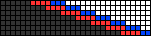
\includegraphics[width=\textwidth]{figs/fdm/unconditional-inference-modes/sample_vis_autoreg_T=30_sampling_3_out_of_7_red_blue_flipped.png}
        \caption{\footnotesize Autoregressive.} \label{fig:autoreg-vis}
    \end{subfigure}
    \begin{subfigure}[t]{0.24\textwidth}
        \centering
        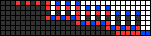
\includegraphics[width=\textwidth]{figs/fdm/unconditional-inference-modes/sample_vis_baby-cond-ho-et-al-for-vis_T=30_sampling_3_out_of_7_red_blue_flipped.png}
        \caption{\footnotesize Two temporal res.} \label{fig:google-vis}
    \end{subfigure}
    \begin{subfigure}[t]{0.24\textwidth}
        \centering
        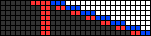
\includegraphics[width=\textwidth]{figs/fdm/unconditional-inference-modes/sample_vis_mixed-autoreg-independent_T=30_sampling_3_out_of_7_red_blue_flipped.png}
        \caption{\footnotesize Long-range (ours).} \label{fig:mixed-vis}
    \end{subfigure}
    \begin{subfigure}[t]{0.24\textwidth}
        \centering
        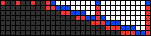
\includegraphics[width=\textwidth]{figs/fdm/unconditional-inference-modes/sample_vis_hierarchy-2_T=30_sampling_3_out_of_7_red_blue_flipped.png}
        \caption{\footnotesize Hierarchy-2 (ours).} \label{fig:hierarchy-vis}
    \end{subfigure}%
    \caption{Sampling schemes that could be used to complete a video of length $N=30$ conditioned on the first 10 frames, with access to at most $K=7$ frames at a time. Each stage $s$ of the sampling procedure is represented by one row in the figure, going from top to bottom. Within each subfigure, one column represents one frame of the video, from frame one on the left to frame 30 on the right. At each stage, the values of frames marked in blue are sampled conditioned on the (observed or previously sampled) values of frames marked in red; frames marked in grey are ignored; and frames marked in white are yet to be sampled. For every sampling scheme, all video frames have been sampled after the final row.
    }
\end{figure*}

Our goal in this paper is to sample coherent photo-realistic videos $\rvv$ with thousands of frames (see \cref{fig:fdm-1}). 
%
To sample an arbitrarily long video with a generative model that can sample or condition on only a small number of frames at once, we must use a sequential procedure. The simplest example of this is an autoregressive scheme, an example of which is shown in \cref{fig:autoreg-vis} for a video completion task. 
%
In this example it takes seven stages to sample a complete video, in that we must run the generative model's sampling procedure seven times. 
%
At each stage three frames are sampled conditioned on the immediately preceding four frames. This scheme is appealing for its simplicity but imposes a strong assumption that, given the set of four frames that are conditioned on at a particular stage, all frames that come afterwards are conditionally independent of all frames that came before. This restriction can be partially ameliorated with the sampling scheme shown in \cref{fig:google-vis} where, in the first three stages, every second frame is sampled and then, in the remaining four stages, the remaining frames are infilled. One way to implement this would be to train two different models operating at the two different temporal resolutions. 
%
In the language of \citet{ho2022video}, who use a similar approach, sampling would be carried out in the first three stages by a ``frameskip-2'' model and, in the remaining stages, by a ``frameskip-1'' model. Both this approach and the autoregressive approach are examples of what we call \textit{sampling schemes}.
%
More generally, we characterise a sampling scheme as a sequence of tuples $[(\mathcal{X}_s, \mathcal{Y}_s)]_{s=1}^S$, each containing a vector $\mathcal{X}_s$ of indices of frames to sample and a vector $\mathcal{Y}_s$ of indices of frames to condition on for stages $s = 1,\ldots,S$. 

\Cref{alg:sampling} lays out how such a sampling scheme is used to sample a video. If the underlying generative model is trained specifically to model sequences of consecutive frames, or sequences of regularly-spaced frames, then the design space for sampling schemes compatible with these models is severely constrained. In this paper we take a  different approach.  We design and train a generative model to sample any arbitrarily-chosen subset of video frames conditioned on any other subset and train it using an entirely novel distribution of such tasks. In short, our model is trained to generate frames for any choice of $\mathcal{X}$ and $\mathcal{Y}$. The only constraint we impose on our sampling schemes is therefore a computational consideration that $|\mathcal{X}_s| + |\mathcal{Y}_s| \leq K$ for all $s$ but, to generate meaningful videos, any valid sampling scheme must also satisfy two more constraints: (1) all frames are sampled at at least one stage and (2) frames are never conditioned upon before they are sampled.

Such a generative model allows us to explore and use sampling schemes like those in \cref{fig:mixed-vis} and \cref{fig:hierarchy-vis}.  We find in our experiments that the best video sampling scheme is dataset dependent. Accordingly, later in this chapter we will present methodology to optimise such sampling schemes in a dataset dependent way, leading to improved video quality as measured by the Fréchet Video Distance~\cite{unterthiner2018towards} among other metrics. We now discuss FDM's architecture, the specific task distribution  used to train it, and the choice and optimisation of sampling schemes in \cref{sec:fdm-architecture}.

\begin{figure*}[t]
    \centering
    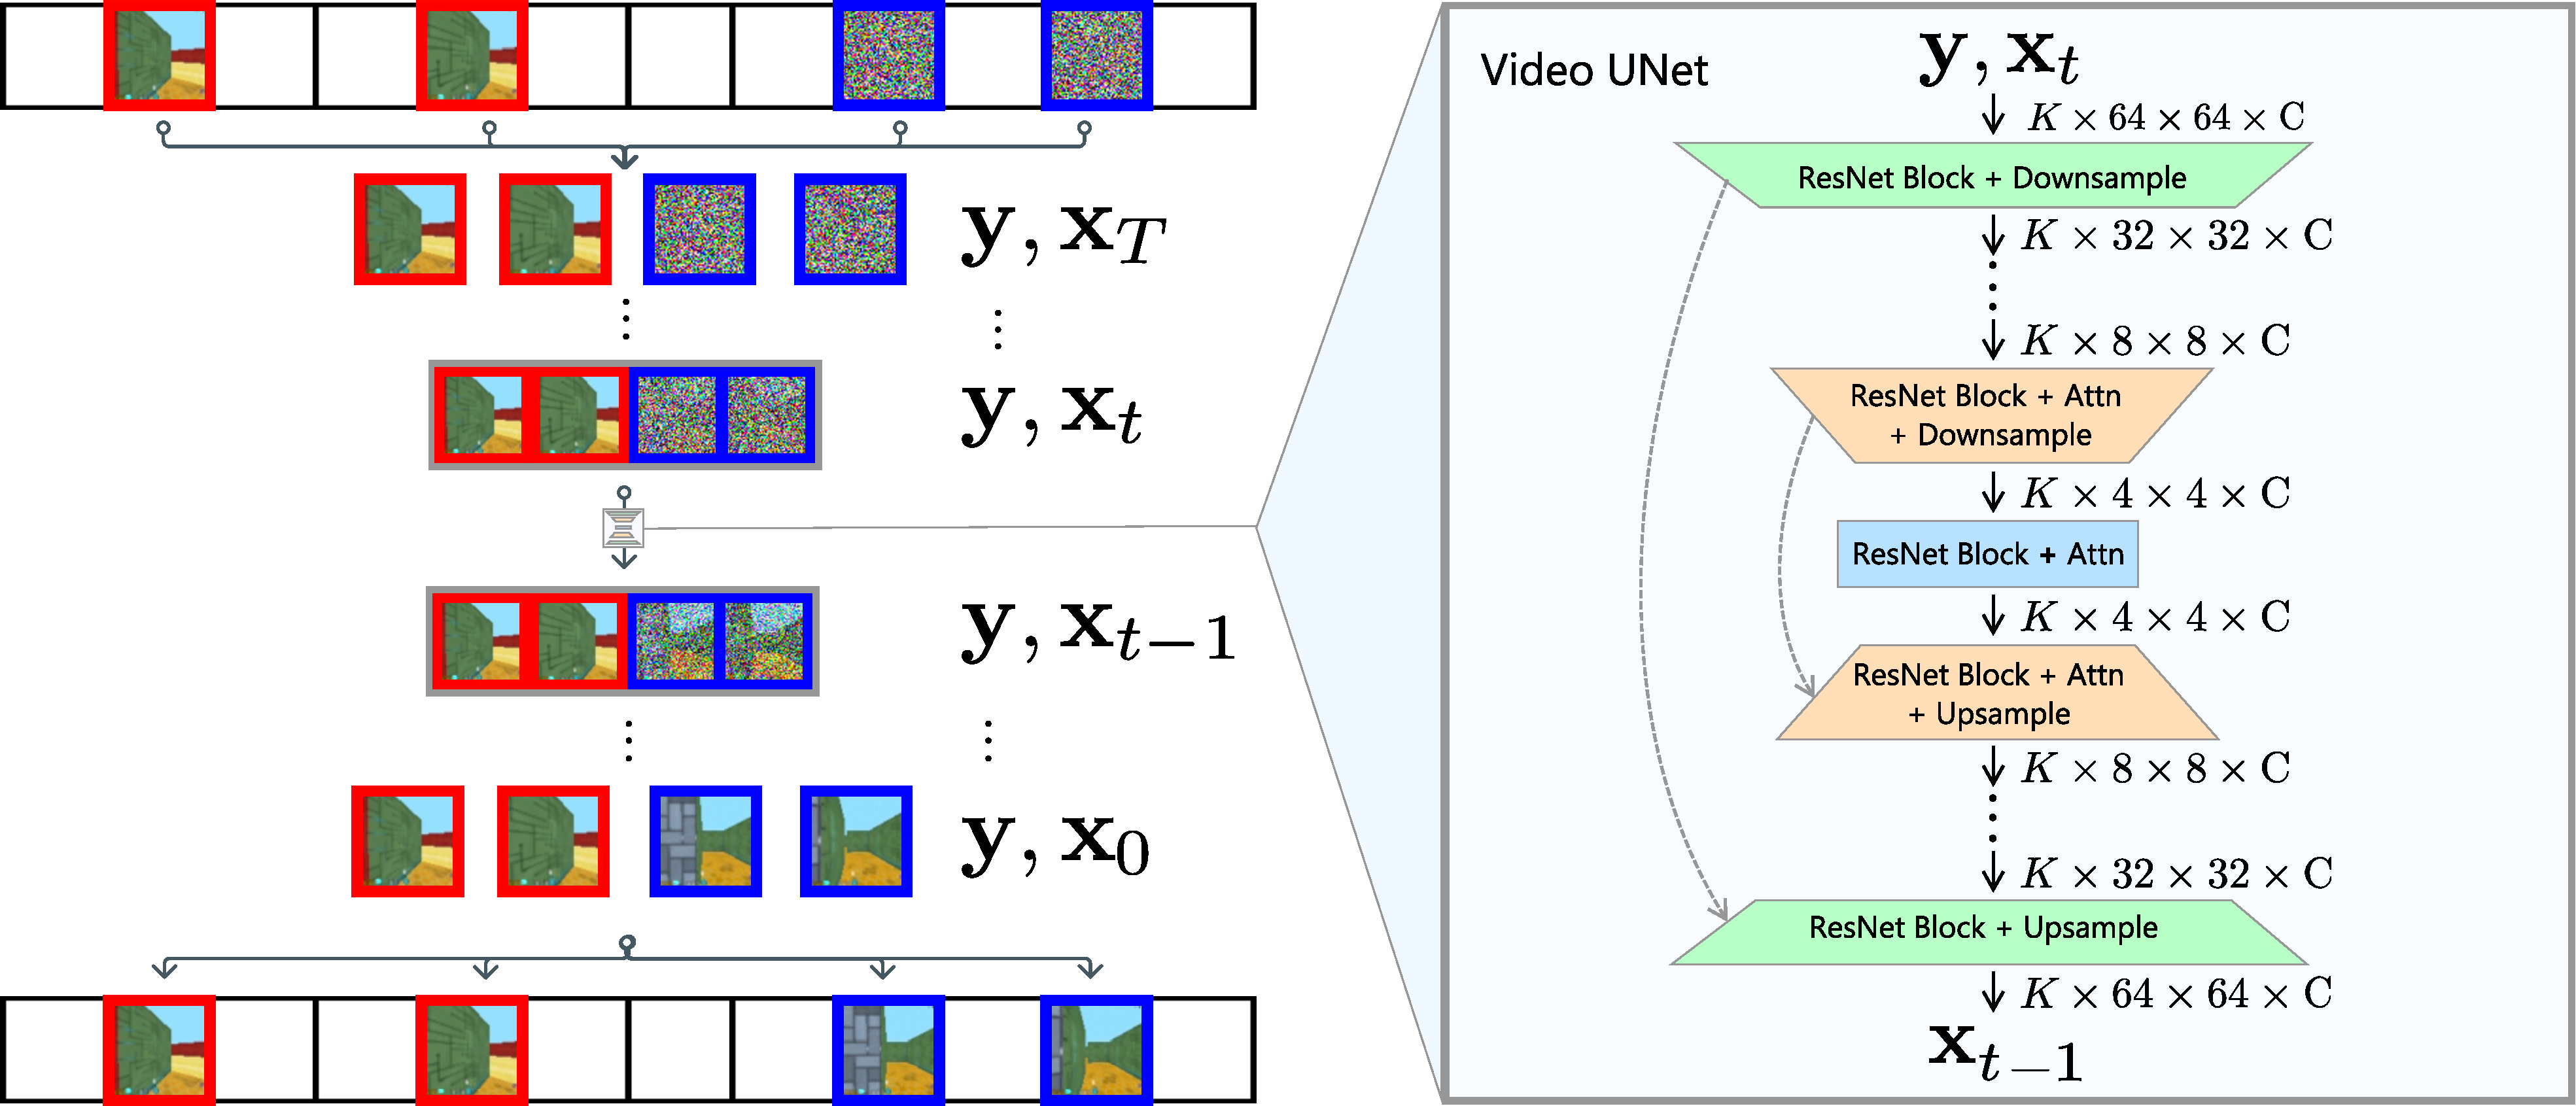
\includegraphics[width=0.88\textwidth]{figs/fdm/video-architecture-v8.pdf}
    \caption{A visualisation of our flexible video diffusion model and its neural architecture. \textbf{Left:} Our DM iteratively transforms Gaussian noise $\rvx_T$ to video frames $\rvx_0$ (shown with blue borders), conditioning on observed frames $\rvy$ (red borders) at every step. \textbf{Right:} The U-net architecture used within each DM step. It computes $\epsilon_\theta(\rvx_t, \rvy, t)$, which is used to transition the state from $\rvx_t$ to $\rvx_{t-1}$ as described in \cref{ch:diffusion}.
    }
    \label{fig:architecture}
\end{figure*}

\section{Training procedure and architecture}\label{sec:fdm-method}

\paragraph{Flexible diffusion objective with marginalisation}
We now present our modification of the flexible diffusion training objective that enables us to vary not just which frames are conditioned on, but also which are generated as opposed to being ``marginalised out''. In \cref{ch:flexible-diffusion} we varied the indices of values to condition on, $\gY$, between training examples, and trained the model to sample all other values. In this chapter we only want the model to sample a subset of the other values so we will introduce, $\gX$, the indices of the values to generate. We will use $\gX$ as an input to the model and vary it between training examples. We rename the original data points $\rvv$ to distinguish them from the objects that the model is trained to generate, $\rvx := \rvv[\gX]$ (i.e. the components of $\rvv$ at indices in $\gX$). We then modify the flexible diffusion objective from \cref{eq:flexible-diffusion-loss} to give the flexible diffusion modelling with marginalisation objective:
\begin{align} \label{eq:fdm-loss}
    \mathcal{L}_\text{FDMM}(\theta) &= 
    % \int_{\sigma_\text{min}}^{\sigma_\text{max}}  
    \EX_{u(\sigma) u(\rvx, \rvx_\sigma, \rvy, \gX, \gY)} \frac{\lambda^\rvx(\sigma)}{u(\sigma)} \left[ 
    \left\| \predx_\theta(\rvx_\sigma, \rvy, \sigma, \gX, \gY) - \rvx \right\|_2^2 \right]
\end{align}
with $u(\rvx, \rvx_\sigma, \rvy, \gX, \gY) = \int u(\gX, \gY)\pdata(\rvv)\delta(\rvx,\rvy|\rvv,\gX,\gY)q(\rvx_\sigma|\rvx) \mathrm{d}\rvv$. We will call $u(\gX, \gY)$ the training task distribution and give a precise specification in the next paragraph ; $\pdata(\rvv)$ is our distribution of long training videos ; $\delta(\rvx,\rvy|\rvv,\gX,\gY)$ is a Dirac distribution which returns $\rvx = \rvv[\gX]$ and $\rvy = \rvv[\gY]$ ; and $q(\rvx_\sigma | \rvx)$ is the standard diffusion ``noising'' distribution as defined in \cref{ch:diffusion}. Recall that, in the standard flexible diffusion setting, the dimensionality of $\rvy$ could vary but that of $\rvx$ was fixed. In the new setting, the dimensionalities of both $\rvx$ and $\rvy$ can vary.

\paragraph{Diffusion process details}
We use variance-preserving diffusion process as described in \cref{sec:more-general-diffusion-processes}, use a discrete-time formulation as described in \cref{sec:diffusion-discrete-time} with 1000 discrete timesteps, and sample with a DDPM-style sampler. See \cref{app:fdm} for full detail.

\paragraph{Training task distribution}
Different choices of latent and observed indices $\mathcal{X}$ and $\mathcal{Y}$ can be regarded as defining different conditional generation tasks. In this sense, we aim to learn a model which can work well on any task (i.e. any choice of $\mathcal{X}$ and $\mathcal{Y}$) and so we randomly sample these vectors of indices during training. We do so with the distribution $u(\latindices,\obsindices)$ described in \cref{fig:training-distribution}. It provides a broad distribution covering many plausible test-time use cases while still providing a better learning signal than a uniform distribution (see ablation in \cref{sec:fdm-experiments} and more details in \cref{ap:fdm-training-task-distribution-ablation}). To cope with constrained computational resources, the distribution is designed such that $|\mathcal{X}|+|\mathcal{Y}|$ is upper-bounded by some pre-specified $K$. Sampling from $q(\rvx, \rvy)$ to compute the our objective (\cref{eq:fdm-loss}) is then accomplished by randomly selecting both a full training video $\rvv$ from the dataset and indices $\mathcal{X},\mathcal{Y}\sim u(\cdot,\cdot)$. We then extract the specified frames $\rvx = \rvv[\latindices]$ and $\rvy = \rvv[\obsindices]$ (where we use $\rvv[\latindices]$ to denote the concatenation of all frames in $\rvv$ with indices in $\latindices$ and and $\rvv[\obsindices]$ similarly).

\begin{figure}
\begin{minipage}[t]{0.33\textwidth}
\begin{figure}[H]
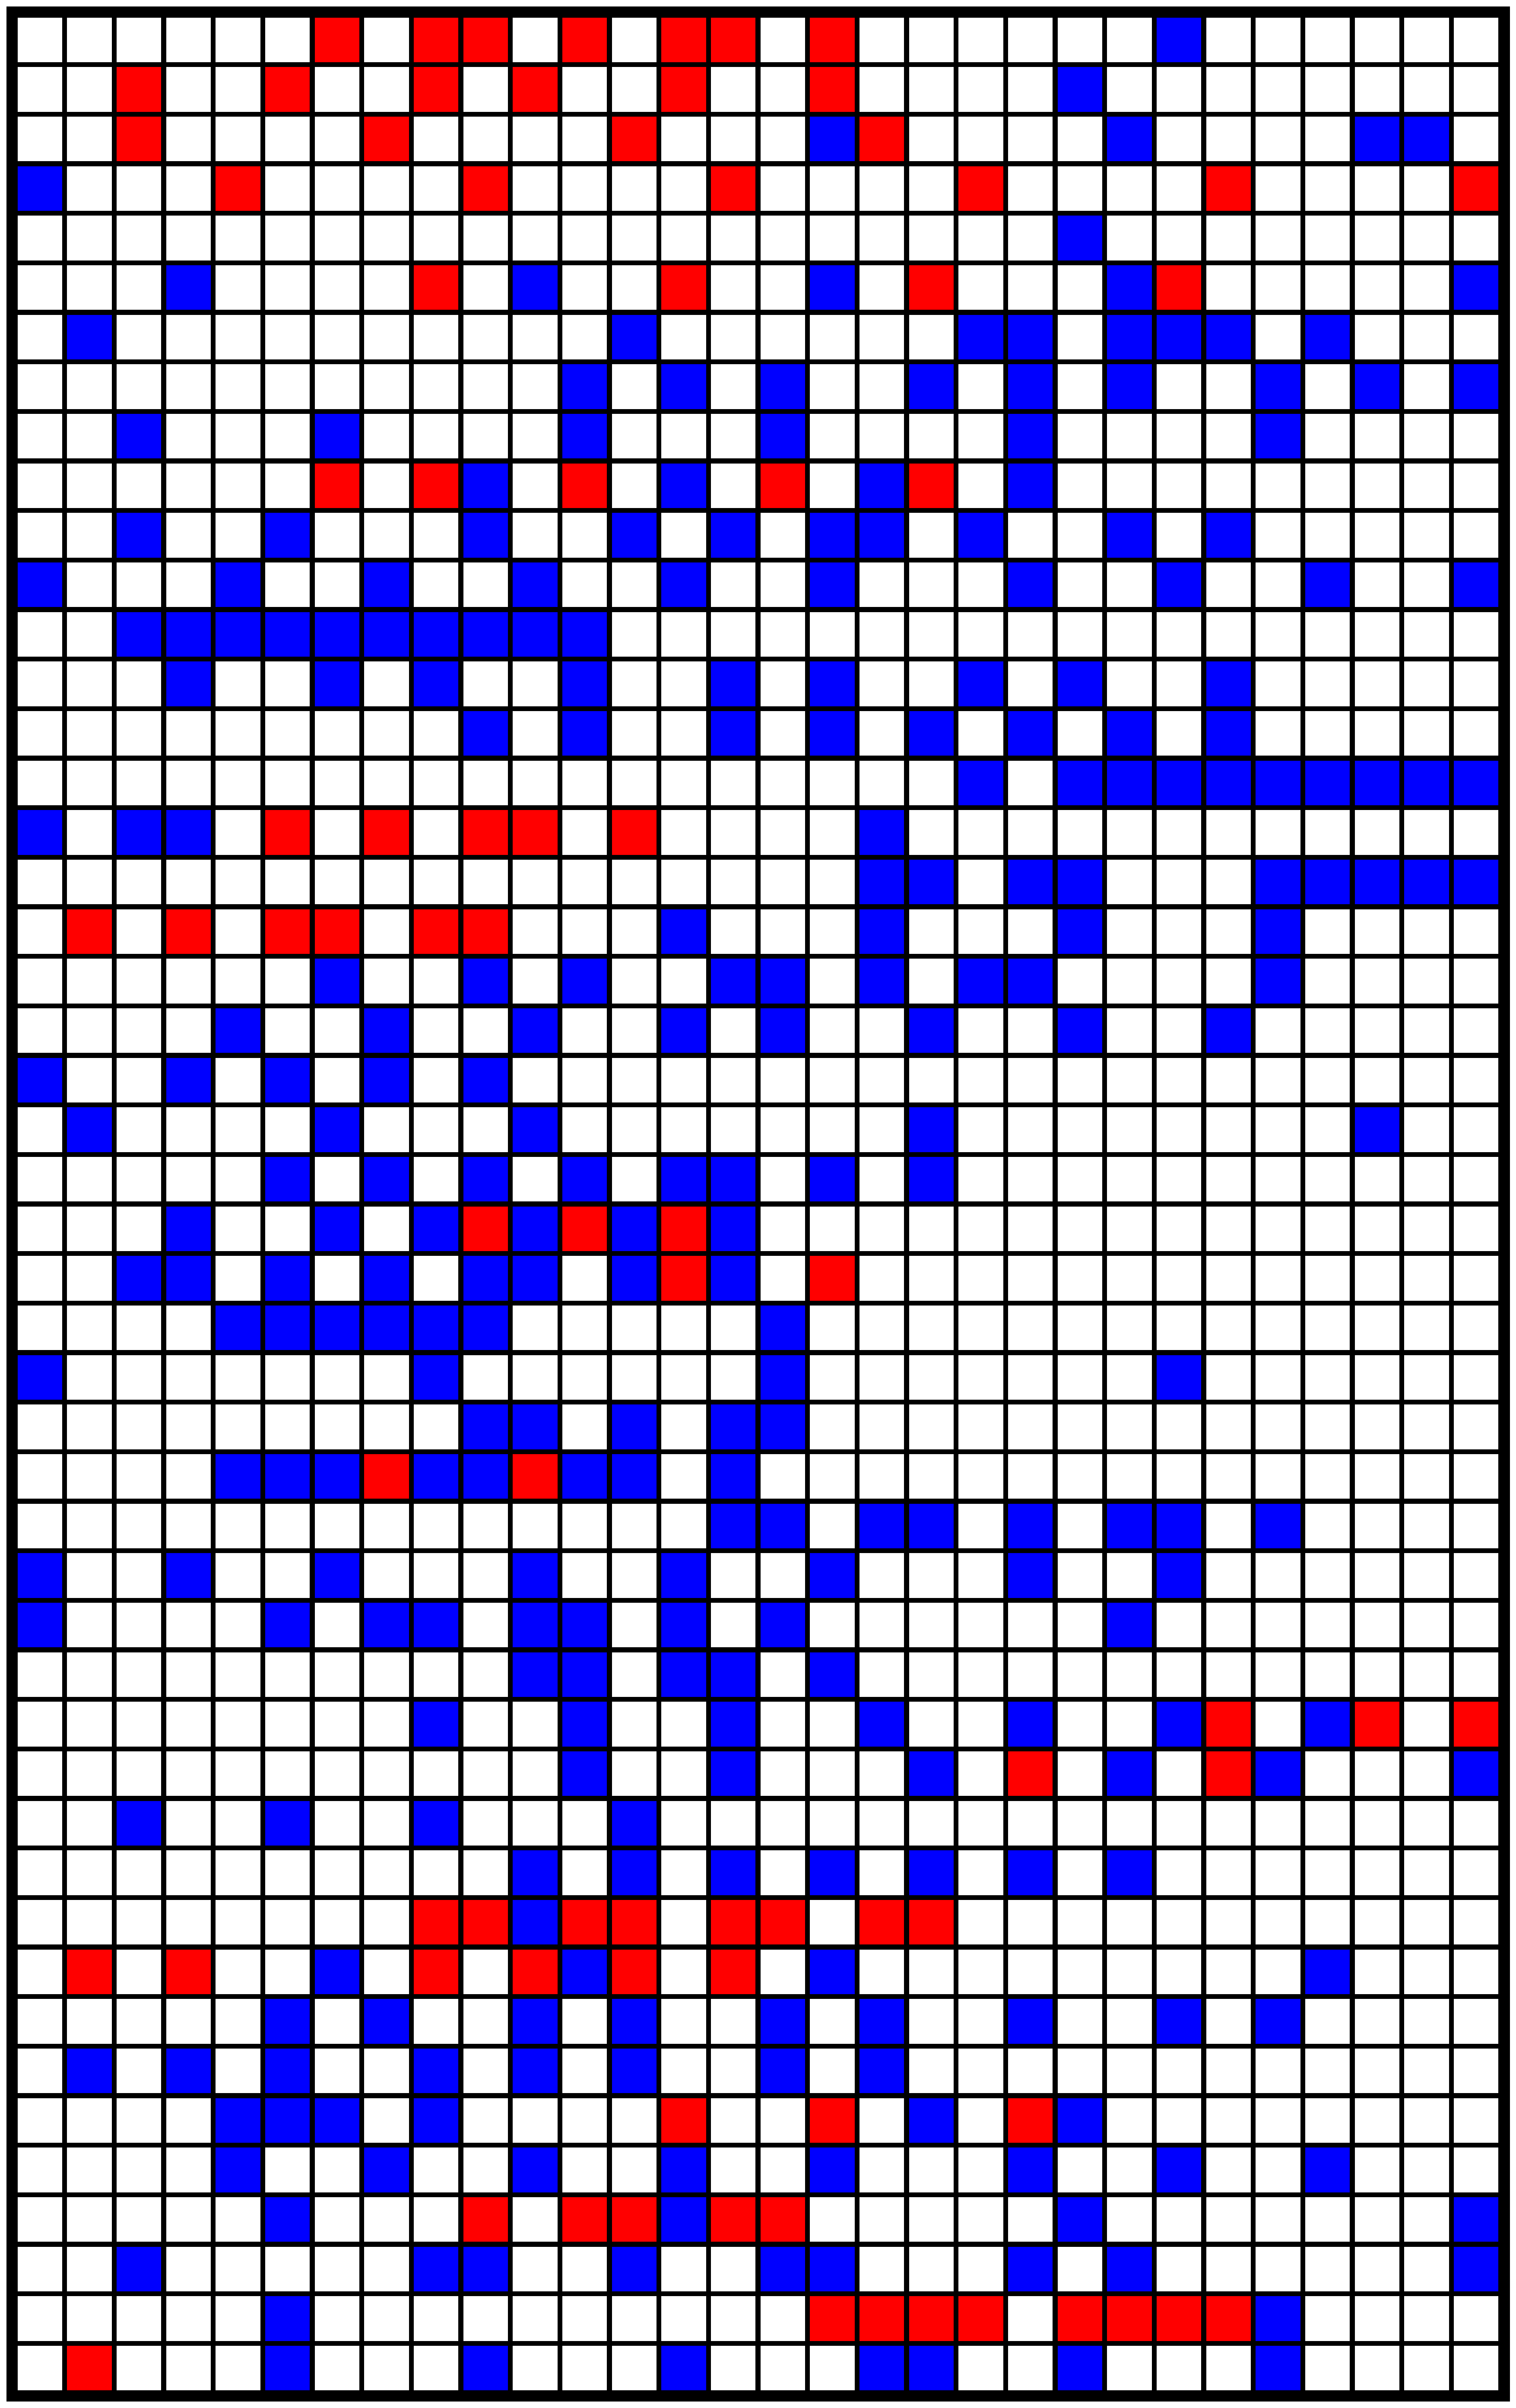
\includegraphics[width=\textwidth]{figs/fdm/training-2.pdf}
\end{figure}
\end{minipage}
\hfill
\begin{minipage}[t]{0.65\textwidth}
\begin{algorithm}[H]
    \caption{Sampling training tasks $\latindices,\obsindices\sim u(\cdot)$ given $N,K$.}\label{alg:mask-distribution}
    \label{alg:training-distribution}
    \footnotesize
    \begin{algorithmic}[1]
      \State $\latindices := \{\}$; $\obsindices := \{\}$
      \While{True}
        \State $n_\text{group} \sim \text{UniformDiscrete}(1, K)$ %\Comment{Sample number of frames in the group}
        \State $s_\text{group} \sim \text{LogUniform}(1, (N-1)/n_\text{group})$ %\Comment{Sample spacing between frames}
        \State $x_\text{group} \sim \text{Uniform}(0, N-(n_\text{group}-1)\cdot s_\text{group})$ %\Comment{Sample position of first frame in the group}
        \State $o_\text{group} \sim \text{Bernoulli}(0.5)$
        \State $\mathcal{G} := \{\lfloor x_\text{group} + s_\text{group} \cdot i \rfloor | i \in \{0,\ldots,n_\text{group}-1\} \} \setminus \latindices \setminus \obsindices$ \label{line:make-G}
        \If{$|\latindices| + |\obsindices| + |\mathcal{G}| > K$}
            \State \Return {$\texttt{set2vector}(\latindices),\texttt{set2vector}(\obsindices)$}
        \ElsIf{$|\latindices| = 0$ \textbf{or} $o_\text{group} = 0$} \label{line:obs-or-lat}
            \State $\latindices := \latindices \cup \mathcal{G}$
        \Else
            \State $\obsindices := \obsindices \cup \mathcal{G}$
        \EndIf
    \EndWhile
    \end{algorithmic}
\end{algorithm}
\end{minipage}
\caption{Samples from our distribution over training tasks, $u(\mathcal{X},\mathcal{Y})$, along with psuedocode for drawing them. \textbf{Left:} Samples with video length $N=30$ and limit $K=10$ on the number of sampled indices. Each row shows one sample and columns map to frames, with frame 1 on the left and frame $N$ on the right. Blue and red denote latent and observed frames respectively. All other frames are ignored and shown as white. \textbf{Right:} Pseudocode for drawing these samples. The while loop iterates over a series of regularly-spaced groups of latent variables. Each group is parameterised by: the number of indices in it, $n_\text{group}$; the spacing between indices in it, $s_\text{group}$; the position of the first frame in it, $x_\text{group}$, and an indicator variable for whether this group is observed, $o_\text{group}$ (which is ignored on line~\ref{line:obs-or-lat} if $\mathcal{X}$ is empty to ensure that the returned value of $\mathcal{X}$ is never empty). These quantities are sampled in a continuous space and then discretised to make a set of integer coordinates on line~\ref{line:make-G}. The process repeats until a group is sampled which, if added to $\latindices$ or $\obsindices$, will cause the number of frames to exceed $K$. That group is then discarded and $\mathcal{X}$ and $\mathcal{Y}$ are returned as vectors. The FDM's training objective forces it to work well for any $(\mathcal{X},\mathcal{Y})$ pair from this broad distribution.
}
\label{fig:training-distribution}
\end{figure}

\paragraph{Architecture}
\label{sec:fdm-architecture}
Image diffusion models~\citep{ho2020denoising,nichol2021improved} typically use a U-net architecture~\cite{ronneberger2015u}. Its distinguishing feature is a series of spatial downsampling layers followed by a series of spatial upsampling layers, and these are interspersed with convolutional ResNet blocks~\cite{he2015deep} and spatial attention layers. Since we require an architecture which operates on 4-D video tensors rather than 3-D image tensors we add an extra \textit{frame} dimension to its input, output and hidden state, resulting in the architecture shown on the right of \cref{fig:architecture}. We create the input to this architecture as a concatenation $\rvx_t \oplus \rvy$, adding an extra input channel which is all ones for observed frames and all zeros for latent frames. For RGB video, the input shape is therefore $(K, \textit{image height}, \textit{image width}, 4)$. Since the output should have the same shape as $\rvx_t$ we only return outputs corresponding to the latent frames, giving output shape  $(|\latindices|, \textit{image height}, \textit{image width}, 3)$. We run all layers from the original model (including convolution, resizing, group normalisation, and spatial attention) independently for each of the $K$ frames.
To allow communication between the frames, we add a temporal attention layer after each spatial attention layer, described in more detail in the appendix. 
%
The spatial attention layer allows each spatial location to attend to all other spatial locations \textit{within} the same frame, while the temporal attention layer allows each spatial location to attend to the same spatial location across all \textit{other} frames.
%
This combination of a temporal attention layer with a spatial attention layer is sometimes referred to as \textit{factorised attention}~\citep{tashiro2021csdi,ho2022video}. We found that, when using this architecture in conjunction with our meta-learning approach, performance could be improved by using a novel form of relative position encoding~\cite{shaw2018self,wu2021rethinking}. We describe this in greater detail in \cref{app:fdm-rpe}.


\paragraph{Training batch padding}
Although the size $|\latindices\oplus\obsindices|$ of index vectors sampled from our training distribution is bounded above by $K$, it can vary. To fit examples with various sizes of index vectors into the same batch, one option would be to pad them all to length $K$ with zeros and use masks so that the zeros cannot affect the loss. This, however, would waste computation on processing tensors of zeros.
%
We instead use this computation to obtain a lower-variance loss estimate by processing additional data with ``training batch padding''.
%
This means that, for training examples where $|\latindices\oplus\obsindices| < K$, we concatenate frames uniformly sampled from a second video to increase the length along the frame-dimension to $K$. Masks are applied to the temporal attention mechanisms so that frames from different videos cannot attend to eachother and the output for each is the same as that achieved by processing the videos in different batches.

\paragraph{Sampling schemes}
Before describing the sampling schemes we experiment with, we emphasise that the relative performance of each is dataset-dependent and there is no single best choice. A central benefit of FDM is that it can be used at test-time with different sampling schemes without retraining. Our simplest sampling scheme, \textbf{Autoreg}, samples ten consecutive frames at each stage conditioned on the previous ten frames. \textbf{Long-range} is similar to Autoreg but conditions on only the five most recent frames as well as five of the original 36 observed frames. \textbf{Hierarchy-2} uses a multi-level sampling procedure. In the first level, ten evenly spaced frames spanning the non-observed portion of the video are sampled (conditioned on ten observed frames). In the second level, groups of consecutive frames are sampled conditioned on the closest past and future frames until all frames have been sampled. \textbf{Hierarchy-3} adds an intermediate stage where several groups of variables with an intermediate spacing between them are sampled. We include Adaptive Hierarchy-2, abbreviated \textbf{Ad. hierarchy-2}, as a demonstration of a sampling scheme only possible with a model like FDM. It samples the same frames at each stage as Hierarchy-2 but selects which frames to condition on adaptively at test-time with a heuristic aimed at collecting the maximally diverse set of frames, as measured by the pairwise LPIPS distance~\cite{zhang2018unreasonable} between them.

\paragraph{Optimising sampling schemes}
An appealing alternative to the heuristic sampling schemes described in the previous paragraph would be to find a sampling scheme that is, in some sense, optimal for a given model and video generation/completion task. While it is unclear how to tractably choose which frames should be sampled at each stage, we suggest that the frames to condition on at each stage can be chosen by greedily optimising the diffusion model loss which, as detailed in \cref{ch:diffusion}, is closely related to the data log-likelihood. Given a fixed sequence of frames to sample at each stage $[\latindices_s]_{s=1}^S$ we select $\obsindices_s$ for each $s$ to minimise the variation of \cref{eq:fdm-loss},
\begin{align}
    % \int_{\sigma_\text{min}}^{\sigma_\text{max}} 
    \EX_{u(\sigma)u(\rvx, \rvx_\sigma, \rvy|\gX_s, \gY_s)} \left[
    \frac{\lambda^\rvx(\sigma)}{u(\sigma)}
    \left\| \predx_\theta(\rvx_\sigma, \rvy, \sigma, \gX_s, \gY_s) - \rvx \right\|_2^2 \right].
\end{align}
This is estimated using a set of 100 training videos and by iterating over 10 evenly-spaced values of $t$ (which reduced variance relative to random sampling of $t$). See the appendix for further details. We create two optimised sampling schemes: one with the same latent indices as Autoreg, and one with the same latent indices as Hierarchy-2. We call the corresponding optimised schemes \textbf{Opt. autoreg} and \textbf{Opt. hierarchy-2}.


\begin{figure}
    \centering
    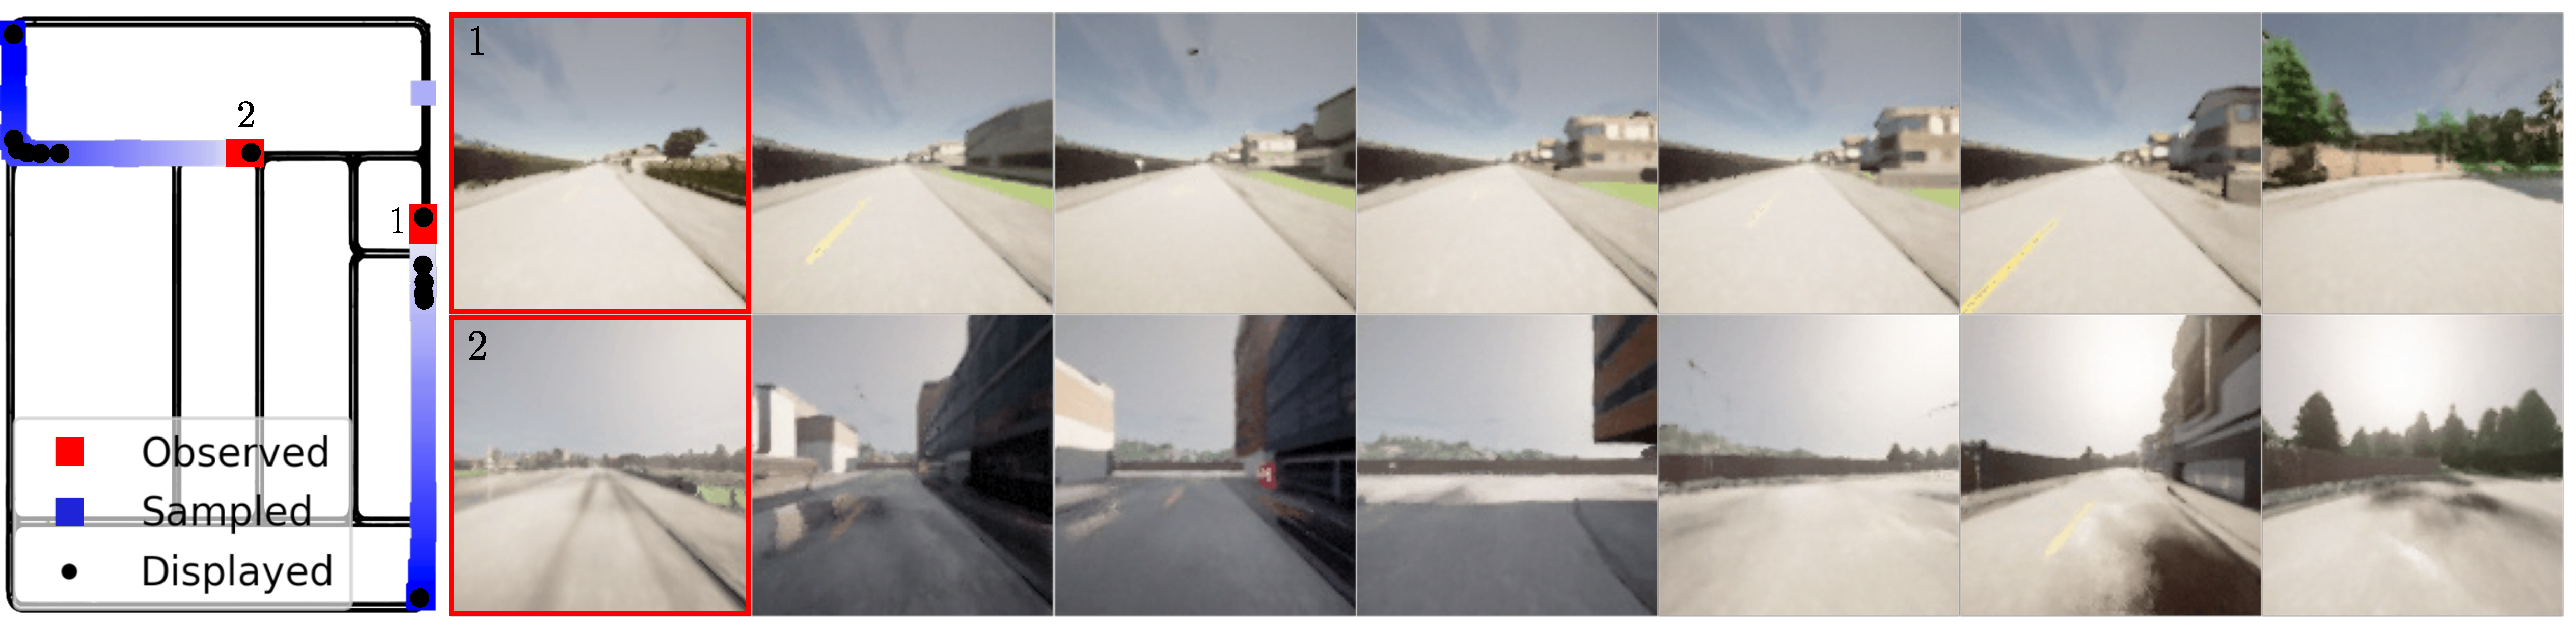
\includegraphics[width=1\textwidth]{figs/fdm/carla_map_7panel}
    \caption{Visualisation of video completions on the CARLA Town01 dataset. \textbf{Left:} Map of the town featured in the CARLA Town01 dataset. We visualise two video completions by FDM by showing coordinates output by our regressor (as discussed in \cref{sec:fdm-carla}) for each frame. Those corresponding to the initial 36 observed frames are shown in red and those for the 964 sampled frames are shown in blue. \textbf{Right:} For each completion, we show one of the initially observed frames followed by four of the sampled frames (at positions chosen to show the progression with respect to visible landmarks and marked by black dots on the map). The town's landmarks are usually sampled with high-fidelity, which is key to allowing the regressor  to produce a coherent trajectory on the left. However there are sometimes failures: a blue square near the top-right of the map shows where the video model ``jumped'' to a wrong location for a single frame.}
    \label{fig:carla}
\end{figure}


\section{CARLA Town01 dataset}
\label{sec:fdm-carla}
In this section we propose a new video modelling dataset and benchmark which provides an interpretable measure of video completion quality. The dataset consists of videos of a car driving with a first-person view, produced using the CARLA autonomous driving simulator~\cite{dosovitskiy2017carla}. All 408 training and 100 test videos (of length 1000 frames and resolution $128\times128$) are produced within a single small town, CARLA's Town01. As such, when a sufficiently expressive video model is trained on this dataset it memorises the layout of the town and videos sampled from the model will be recognisable as corresponding to routes travelled within the town. We train a regression model in the form of a neural network which maps with high accuracy from any single rendered frame to $(x,y)$ coordinates representing the car's position. Doing so allows us to plot the routes corresponding to sampled videos (see left of \cref{fig:carla}) and compute semantically-meaningful yet quantitative measures of the validity of these routes. Specifically, we compute histograms of speeds, where each speed is estimated by measuring the distance between the regressed locations for frames spaced ten apart (1 second at the dataset's frame rate). Sampled videos occasionally ``jump'' between disparate locations in the town, resulting in unrealistically large estimated speeds. To measure the frequency of these events for each method, we compute the percentage of our point-speed estimates that exceed a threshold of $10$m/s (the dataset was generated with a maximum simulated speed of $3$m/s). We report this metric as the outlier percentage (OP). After filtering out these outliers, we compute the Wasserstein distance (WD) between the resulting empirical distribution and that of the original dataset, giving a measure of how well the speeds in generated videos match the speeds in dataset videos. We have released the CARLA Town01 dataset and trained regression model along with the rest of our code to allow future comparisons.\footnote{\url{https://github.com/plai-group/flexible-video-diffusion-modeling}}

\section{Experiments} \label{sec:fdm-experiments}

We perform our main comparisons on the video completion task. For this task, in keeping with \citet{saxena2021clockwork}, we condition on the first 36 frames of each video and sample the remainder. We present results on three datasets: GQN-Mazes~\citep{eslami2018neural}, in which videos are 300 frames long; MineRL Navigate~\citep{guss2019minerl,saxena2021clockwork} (which we will from now on refer to as simply MineRL), in which videos are 500 frames long; and the CARLA Town01 dataset we release, for which videos are 1000 frames long. We train FDM in all cases with the maximum number of represented frames $K=20$. We host non-cherry-picked video samples (both conditional and unconditional) from FDM and baselines online\footnote{\url{https://www.cs.ubc.ca/~wsgh/fdm}}.


\begin{table*}
  \scriptsize
  \caption{Evaluation of video completions by our method (FDM) with various sampling schemes along with several baselines from the literature. Error bars denote the standard error computed with 5 random seeds. Higher is better for the accuracy metric~\cite{saxena2021clockwork} and lower is better for all other metrics shown.}
  \label{tab:fdm-results-completion}
  \centering
  \begin{tabular}{llllllll}
    \toprule
    \multicolumn{1}{r}{} & & \multicolumn{2}{c}{GQN-Mazes}  & \multicolumn{1}{c}{MineRL}  & \multicolumn{3}{c}{CARLA Town01} \\
    \cmidrule(r){3-4} \cmidrule(r){5-5} \cmidrule(r){6-8}
    Model &  Sampling scheme        & FVD      & Accuracy  & FVD     &  FVD     & WD  & OP \\
    \midrule
    \multirow{1}{*}{CWVAE~\citep{saxena2021clockwork}}
    & CWVAE  & $837 \pm 8$      & $82.6 \pm 0.5$  & $1573 \pm 5$                 & $1161$          & $0.666$   & $44.4$        \\
    \midrule
    \multirow{1}{*}{TATS~\citep{ge2022long}}
    & TATS   & $163 \pm 2.6$  &  $77.0 \pm 0.8$  & $807 \pm 14$          & $329$          & $1.648$          & $42.4$ \\
    \midrule
    \multirow{1}{*}{VDM~\citep{ho2022video}}
    & VDM   & $66.7 \pm 1.5$  &  $77.8 \pm 0.5$  & $271 \pm 8.8$          & $169$          & $0.501$          & $16.9$ \\
    \midrule
    \multirow{5}{*}{FDM (ours)}
    &  Autoreg        & $86.4 \pm 5.2$          & $69.6 \pm 1.3$   & $281 \pm 10$          & $222$          & $0.579$      & $0.51$     \\
    &  Long-range           & $64.5\pm1.9$            & $77.0 \pm 1.4$   & $\mathbf{267 \pm 4.0}$     & $213$          & $0.653$      & $\mathbf{0.47}$     \\
    &  Hierarchy-2          & $\mathbf{53.1 \pm 1.1}$ & $82.8 \pm 0.7$   & $275 \pm 7.7$        & $120$     & $0.318$  &  $3.28$      \\
    &  Hierarchy-3          & $53.7 \pm 1.9$          & $\mathbf{83.8 \pm 1.1}$   & $311 \pm 6.8$        & $149$      & $0.363$    &  $4.53$  \\
    &  Ad. hierarchy-2      & $55.0 \pm 1.4$          & $83.2 \pm 1.3$   & $316 \pm 8.9$    & $\mathbf{117}$          & $\mathbf{0.311}$     & $3.44$    \\
    \bottomrule
  \end{tabular}
\end{table*}

\paragraph{Comparison of sampling schemes}
\begin{figure}
    \centering
    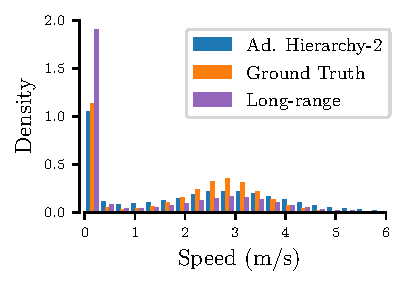
\includegraphics[width=0.6\textwidth]{figs/fdm/hist_new.pdf}
    \caption{Comparison of speed distributions measured from dataset videos with those measured from videos sampled by our model using two different sampling schemes. The ground-truth speeds are concentrated around $3m/s$ with some additional probability mass on zero. Videos sampled with Long-range have more mass at zero than is realistic. Sampling with Ad. Hierarchy-2 fixes this problem, although neither sampling scheme is as concentrated around $3m/s$ as the ground truth.}
    \label{fig:hist}
\end{figure}
The relative performance of different sampling schemes varies significantly between datasets as shown in \cref{tab:fdm-results-completion}. We report Fréchet Video Distances (FVDs)~\cite{unterthiner2018towards}, a measure of how similar sampled completions are to the test set, on all datasets. In addition on GQN-Mazes we we report the accuracy metric~\cite{saxena2021clockwork}, which classifies videos based on which rooms are visited and measures how often a completion is given the same class as the corresponding test video. For CARLA Town01 we report the previously described percentage outliers (PO) and Wasserstein distance (WD) metrics. 

We can broadly consider the aforementioned sampling schemes as either being in the ``autoregressive'' family (Autoreg and Long-range) or in the ``hierarchical'' family (the remainder). Those in the hierarchical family achieve significantly better FVDs~\cite{unterthiner2018towards} on GQN-Mazes. Our samples in the appendix suggest that this is related to the autoregressive methods ``forgetting'' the colours of walls after looking away from them for a short time. In contrast, for MineRL the autoregressive methods tend to achieve the best FVDs. This may relate to the fact that trajectories in MineRL tend to travel in straight lines through procedurally-generated ``worlds''\cite{guss2019minerl,saxena2021clockwork}, limiting the number of long-range dependencies. 
Finally on CARLA Town01 we notice qualitatively different behaviours from our autoregressive and hierarchical sampling schemes. The hierarchical
sampling schemes have a tendency to occasionally lose coherence and ``jump'' 
to different locations in the town. This is reflected by higher outlier percentages (OP) in \cref{tab:fdm-results-completion}. On the other hand the autoregressive schemes often stay stationary for unrealistically long times at traffic lights. This is reflected in the histogram of speeds in \cref{fig:hist}, which has a larger peak around zero than the ground truth. The high variance of the sampling scheme's relative performance over different datasets points to a strength of our method, which need only be trained once and then used to explore a variety of sampling schemes. Furthermore, we point out that the best FVDs in \cref{tab:fdm-results-completion} on all datasets were obtained using sampling schemes that could not be implemented using models trained in prior work, or over evenly spaced frames.

\paragraph{Comparison with baselines}
The related work most relevant to ours is the concurrent work of \citet{ho2022video}, who model 64-frame videos using two trained DMs. The first is a ``frameskip-4'' model trained to generate every fourth frame and the second is a ``frameskip-1'' model trained on sequences of nine consecutive frames and used to ``fill in'' the gaps between frames generated in the first stage. To compare against this approach, which we denote \textbf{VDM}, we train both a ``frameskip-4'' and a ``frameskip-1'' model with architectures identical to our own.\footnote{The VDM is concurrent work and, at the time of writing, without a code-release. Since we intend this primarily as a comparison against the VDM sampling scheme we do not reimplement their exact architecture and note that there are other differences including their approach to imputation.} Since VDM requires two trained DMs, we train it for more GPU-hours than FDM despite the fact that FDM is meta-learning over a far broader task distribution. We also compare against \textbf{TATS}~\citep{ge2022long}, which embeds videos into a discrete latent space before modelling them with a transformers, and the clockwork VAE (\textbf{CWVAE})~\citep{saxena2021clockwork}, a VAE-based model specifically designed to maintain long-range dependencies within video.

Both the diffusion-based methods, FDM and VDM, achieve significantly higher FVD scores than TATS and CWVAE. This may point toward the utility of diffusion models in general for modelling images and video. \Cref{tab:fdm-results-completion} also makes clear the main benefit of FDM over VDM: although there is no sampling scheme for FDM which always outperforms VDM, there is at least one sampling scheme that outperforms it on each dataset. This speaks to the utility of learning a flexible model like FDM that allows different sampling schemes to be experimented with after training.

\begin{table} %{r}{80mm}
  \small
  \caption{Evaluation of video completions by our method with sampling schemes optimised offline as described in \cref{sec:fdm-method}.  We mark with an asterisk ($^*$) the eight numbers which improve on the corresponding non-optimised sampling schemes and highlight in bold those that are better than any in \cref{tab:fdm-results-completion}.}
  \vspace{2mm}
  \label{tab:fdm-optimized}
  \centering
  \begin{tabular}{lllllllll}
    \toprule
     & \multicolumn{2}{c}{GQN-Mazes}  & \multicolumn{1}{c}{MineRL}  & \multicolumn{3}{c}{CARLA Town01} \\
    \cmidrule(r){2-3} \cmidrule(r){4-4} \cmidrule(r){5-7}
    Sampling scheme       & FVD     & Accuracy    &    FVD & FVD & WD & OP \\
    \midrule
    Opt. autoreg        & $53.6 \pm 1.2^*$            & $80.2 \pm 1.2^*$            & $\mathbf{257 \pm 6.8}^*$    &   $146^*$ & $0.452^*$ & $0.65$   \\
    Opt. hierarchy-2   & $\mathbf{51.1 \pm 1.3}^*$    & $\mathbf{84.6 \pm 0.7}^*$   & $320 \pm 7.0$    &   $124$ & $0.349$ & $4.11^*$   \\
    \bottomrule
  \end{tabular}
\end{table}

\paragraph{Optimised sampling schemes}
As mentioned in \cref{sec:fdm-method}, another advantage of FDM is that it makes possible a model- and dataset-specific optimisation procedure to determine which frames to condition on at each stage. \Cref{tab:fdm-optimized} shows the results when this procedure is used to create sampling schemes for different datasets. In the first row we show results where the latent frames are fixed to be those of the Autoreg sampling scheme, and in the second row the latent frames are fixed to match those of Hierarchy-2. On two of the three datasets the best results in \cref{tab:fdm-results-completion} are improved upon, showing the utility of this optimisation procedure.

\paragraph{Comparison with training on a single task}
Training a network with our distribution over training tasks could be expected to lead to worse performance on a single task than training specifically for that task. To test whether this is the case, we train an ablation of FDM with training tasks exclusively of the type used in our Autoreg sampling scheme, i.e. ``predict ten consecutive frames given the previous ten.'' Tested with the Autoreg sampling scheme, it obtained an FVD of $82.0$ on GQN-Mazes and $234$ on MineRL. As expected given the specialisation to a single task, this is better than when FDM is run with the Autoreg sampling scheme (obtaining FVDs of $86.4$ and $281$ respectively).

\paragraph{Ablation on training task distribution}
To test how important our proposed structured training distribution is to FDM's performance, we perform an ablation with a different task distribution that samples $\latindices$ and $\obsindices$ from uniform distributions instead of our proposed structured task distribution. 
We provide full details in the appendix, but report here that switching away form our structured training distribution made the FVD scores worse on all five tested sampling schemes on both GQN-Mazes and MineRL. The reduction in the average FVD was $31\%$ on GQN-Mazes and $52\%$ on MineRL. This implies that our structured training distribution has a significant positive effect.

\section{Related work}


There are a number of approaches in the literature which use VAEs rather than DMs for video modelling. \citet{babaeizadeh2017stochastic} use a VAE model which predicts frames autoregressively conditioned on a global time-invariant latent variable. A related approach by \citet{denton2018stochastic} also uses a VAE with convolutional LSTM architectures in both the encoder and decoder. Unlike \citet{babaeizadeh2017stochastic} the prior is learned and a different latent variable is sampled for each frame. \citet{babaeizadeh2021fitvid} use a VAE with one set of latent variables per frame and inter-frame dependencies tracked by a two-layer LSTM. Their architecture intentionally overfits to the training data, which when coupled with image augmentations techniques achieves SOTA on various video prediction tasks.  \citet{kim2019variational} use a variational RNN~\citep{chung2015recurrent} with a hierarchical latent space that includes binary indicator variables which specify how the video is divided into a series of subsequences. Both \citet{villegas2018hierarchical} and \citet{wichers2018learning} target long-term video prediction using a hierarchical variational LSTM architecture, wherein high-level features such as landmarks are predicted first, then decoded into low-level pixel space. The two approaches differ in that \citet{villegas2018hierarchical} requires ground truth landmark labels, while \cite{wichers2018learning} removes this dependence using an unsupervised adversarial approach. Fully GAN-based video models have also been proposed~\citep{aldausari2022video,clark2019adversarial} but generally suffer from ``low quality frames or low number of frames or both''~\citep{aldausari2022video}.

\section{Discussion}
%Our method is still slow to sample from. There are techniques to speed up sampling~\citep{salimans2022progressive,song2020denoising} but exploring them was outside the scope of this paper.

In this chapter we have defined and empirically explored a new method for generating photorealistic videos with long-range coherence that respects and efficiently uses fixed, finite computational resources.
Our approach outperforms prior work on long-duration video modelling as measured by quantitative and semantically meaningful metrics. By doing so it serves as evidence that, when our data is sufficiently complex and high-dimensional, the flexible diffusion framework and flexible generative models can be useful for creating better generative models even if we only care about a single task like video continuation. In addition, the model we have presented is applicable to far more tasks without further training. Such tasks include conditioning on every $n$th frame to enable temporal super-resolution, or conditioning on both the first and final frame (potentially yielding a ``visual'' controller which proposes a path between a current state and a specified goal). Preliminary attempts to run in FDM conditioned on a final frame in this way yielded inconsistent results but we believe that this could be a fruitful direction for further investigation. Another promising avenue for exploration is simply to design better sampling schemes. More automated techniques to optimise these sampling schemes, and even to make them adapt given the values of previously generated frames, could have further benefits. One limitation of FDM is that each frame it considers must be either fully observed or fully unobserved; this was acceptable for the tasks we considered but more recent work has found that removing this limitation enables new inpainting-style tasks~\citep{green2024semantically}.
